% Tidal Forces and Geodesic Deviation
% File: tikz_tidal_forces.tex
% Purpose: Visualize geodesic deviation equation and tidal effects
% For: Chapter 1 - Mathematical Preliminaries

\begin{figure}[htbp]
\centering
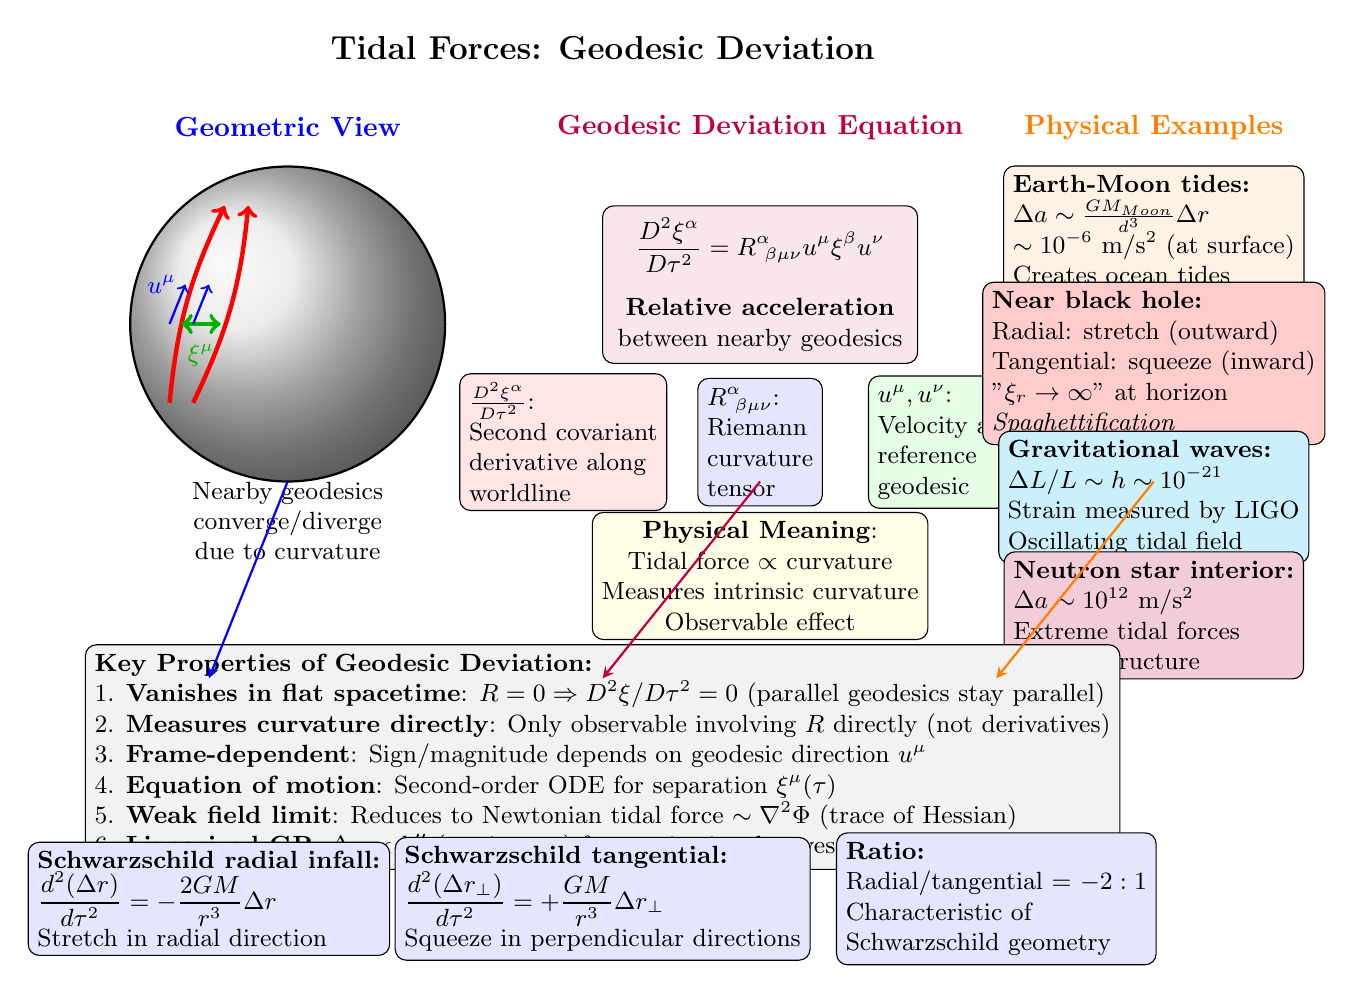
\begin{tikzpicture}[scale=1.0, every node/.style={font=\small}]

% Title
\node[font=\bfseries\large] at (7, 7.5) {Tidal Forces: Geodesic Deviation};

% Left panel: Geometric picture
\begin{scope}[shift={(0,0)}]
    \node[font=\bfseries, blue] at (3, 6.5) {Geometric View};
    
    % Curved surface (sphere segment)
    \shade[ball color=gray!20] (3, 4) circle (2cm);
    \draw[thick] (3, 4) circle (2cm);
    
    % Two nearby geodesics
    \draw[red, ultra thick, ->] (1.5, 3) to[bend left=10] (2.2, 5.5);
    \draw[red, ultra thick, ->] (1.8, 3) to[bend right=10] (2.5, 5.5);
    
    % Separation vector
    \draw[green!70!black, ultra thick, <->] (1.65, 4) -- (2.15, 4);
    \node[green!70!black] at (1.9, 3.6) {$\xi^\mu$};
    
    % Tangent vectors
    \draw[blue, thick, ->] (1.5, 4) -- (1.7, 4.5);
    \draw[blue, thick, ->] (1.8, 4) -- (2.0, 4.5);
    \node[blue] at (1.4, 4.5) {$u^\mu$};
    
    % Curvature annotation
    \node[align=center] at (3, 1.5) {
        Nearby geodesics\\
        converge/diverge\\
        due to curvature
    };
\end{scope}

% Center panel: Equation
\begin{scope}[shift={(6,0)}]
    \node[font=\bfseries, purple] at (3, 6.5) {Geodesic Deviation Equation};
    
    % Main equation box
    \node[draw, fill=purple!10, align=center, rounded corners, minimum width=4cm, minimum height=2cm] at (3, 4.5) {
        $\displaystyle \frac{D^2 \xi^\alpha}{D\tau^2} = R^\alpha_{\ \beta\mu\nu} u^\mu \xi^\beta u^\nu$\\[0.3cm]
        \textbf{Relative acceleration}\\
        between nearby geodesics
    };
    
    % Component breakdown
    \node[draw, fill=red!10, align=left, rounded corners] at (0.5, 2.5) {
        $\frac{D^2 \xi^\alpha}{D\tau^2}$:\\
        Second covariant\\
        derivative along\\
        worldline
    };
    
    \node[draw, fill=blue!10, align=left, rounded corners] at (3, 2.5) {
        $R^\alpha_{\ \beta\mu\nu}$:\\
        Riemann\\
        curvature\\
        tensor
    };
    
    \node[draw, fill=green!10, align=left, rounded corners] at (5.5, 2.5) {
        $u^\mu, u^\nu$:\\
        Velocity along\\
        reference\\
        geodesic
    };
    
    % Physical meaning
    \node[draw, fill=yellow!10, align=center, rounded corners] at (3, 0.8) {
        \textbf{Physical Meaning}:\\
        Tidal force $\propto$ curvature\\
        Measures intrinsic curvature\\
        Observable effect
    };
\end{scope}

% Right panel: Tidal examples
\begin{scope}[shift={(11,0)}]
    \node[font=\bfseries, orange] at (3, 6.5) {Physical Examples};
    
    % Earth-Moon system
    \node[draw, fill=orange!10, align=left, rounded corners] at (3, 5.2) {
        \textbf{Earth-Moon tides:}\\
        $\Delta a \sim \frac{GM_{\text{Moon}}}{d^3} \Delta r$\\
        $\sim 10^{-6}$ m/s$^2$ (at surface)\\
        Creates ocean tides
    };
    
    % Spaghettification
    \node[draw, fill=red!20, align=left, rounded corners] at (3, 3.5) {
        \textbf{Near black hole:}\\
        Radial: stretch (outward)\\
        Tangential: squeeze (inward)\\
        "$\xi_r \to \infty$" at horizon\\
        \emph{Spaghettification}
    };
    
    % LIGO
    \node[draw, fill=cyan!20, align=left, rounded corners] at (3, 1.8) {
        \textbf{Gravitational waves:}\\
        $\Delta L / L \sim h \sim 10^{-21}$\\
        Strain measured by LIGO\\
        Oscillating tidal field
    };
    
    % Neutron star
    \node[draw, fill=purple!20, align=left, rounded corners] at (3, 0.3) {
        \textbf{Neutron star interior:}\\
        $\Delta a \sim 10^{12}$ m/s$^2$\\
        Extreme tidal forces\\
        Affects structure
    };
\end{scope}

% Bottom: Mathematical details
\node[draw, fill=gray!10, align=left, rounded corners] at (7, -1.5) {
    \textbf{Key Properties of Geodesic Deviation:}\\
    1. \textbf{Vanishes in flat spacetime}: $R = 0 \Rightarrow D^2\xi/D\tau^2 = 0$ (parallel geodesics stay parallel)\\
    2. \textbf{Measures curvature directly}: Only observable involving $R$ directly (not derivatives)\\
    3. \textbf{Frame-dependent}: Sign/magnitude depends on geodesic direction $u^\mu$\\
    4. \textbf{Equation of motion}: Second-order ODE for separation $\xi^\mu(\tau)$\\
    5. \textbf{Weak field limit}: Reduces to Newtonian tidal force $\sim \nabla^2 \Phi$ (trace of Hessian)\\
    6. \textbf{Linearized GR}: $\Delta a \propto h''$ (strain rate) for gravitational waves
};

% Schwarzschild specific formula
\node[draw, fill=blue!10, align=left, rounded corners] at (2, -3.3) {
    \textbf{Schwarzschild radial infall:}\\
    $\displaystyle \frac{d^2(\Delta r)}{d\tau^2} = -\frac{2GM}{r^3} \Delta r$\\
    Stretch in radial direction
};

\node[draw, fill=blue!10, align=left, rounded corners] at (7, -3.3) {
    \textbf{Schwarzschild tangential:}\\
    $\displaystyle \frac{d^2(\Delta r_\perp)}{d\tau^2} = +\frac{GM}{r^3} \Delta r_\perp$\\
    Squeeze in perpendicular directions
};

\node[draw, fill=blue!10, align=left, rounded corners] at (12, -3.3) {
    \textbf{Ratio:}\\
    Radial/tangential = $-2:1$\\
    Characteristic of\\
    Schwarzschild geometry
};

% Connecting lines
\draw[->, >=stealth, thick, blue] (3, 2) -- (2, -0.5);
\draw[->, >=stealth, thick, purple] (9, 2) -- (7, -0.5);
\draw[->, >=stealth, thick, orange] (14, 2) -- (12, -0.5);

\end{tikzpicture}
\caption{Tidal forces as manifestation of spacetime curvature through geodesic deviation equation. Left: Geometric picture showing two nearby geodesics with separation vector $\xi^\mu$ that accelerates relative to reference geodesic with velocity $u^\mu$. Center: Geodesic deviation equation $D^2\xi^\alpha/D\tau^2 = R^\alpha_{\ \beta\mu\nu} u^\mu \xi^\beta u^\nu$ relating relative acceleration to Riemann curvature. Right: Physical examples from ocean tides ($10^{-6}$ m/s$^2$) to black hole spaghettification to LIGO strain measurements ($10^{-21}$) to neutron star interiors ($10^{12}$ m/s$^2$). Bottom: Mathematical properties and Schwarzschild-specific formulas showing characteristic 2:1 stretch-squeeze ratio. Geodesic deviation provides direct observable measurement of curvature.}
\label{fig:tidal_forces}
\end{figure}
